\chapter{Fundamental Concepts and Solution Chemistry}
\label{ch:fundamental_concepts}

\begin{chapterintro}
\textbf{Chapter Objectives:} In this foundational chapter, we establish the quantitative and macroscopic framework of chemical science. You will master the macroscopic states of matter and phase change thermodynamics; formulate Lavoisier's conservation principle; manipulate amount of substance using Avogadro's number; define atomic and molar mass metrics; systematically classify pure substances and mixtures; and derive rigorous expressions for solution concentrations---molarity, mass concentration, molality, and normality across acid-base and redox reactions.
\end{chapterintro}

\section{States and Macroscopic Properties of Matter}

\begin{definitionbox}{Matter}
\textbf{Matter} is formally defined as any physical entity that possesses inertial mass ($m$) and occupies a finite spatial volume ($V$). The quantitative measure of its spatial compactness is its \textbf{mass density} (volumetric mass):
\begin{equation}
\rho \eqdef \frac{m}{V}, \qquad [\rho] = \mathrm{kg\cdot m^{-3}} \quad (\text{or } \mathrm{g\cdot cm^{-3}} = \mathrm{g\cdot mL^{-1}}).
\end{equation}
\end{definitionbox}

Under standard environmental conditions, matter organizes into three classical macroscopic physical states governed by the balance between thermal kinetic energy ($\sim k_B T$) and cohesive intermolecular forces:

\begin{itemize}[leftmargin=1.5em,itemsep=4pt]
  \item \textbf{Solid State:} Possesses both a \textbf{definite, fixed volume} and a \textbf{definite geometric shape}. The constituent particles (atoms, ions, or molecules) are locked into fixed spatial coordinates by powerful intermolecular or ionic bonds, executing only small-amplitude thermal vibrations about their equilibrium lattice sites. Solids exhibit high resistance to shear deformations and are virtually incompressible.
  \item \textbf{Liquid State:} Possesses a \textbf{definite, fixed volume}, but \textbf{no fixed shape}; it deforms continuously under shear stress to adopt the geometric contours of its container while maintaining a well-defined free surface in gravity. The intermolecular attractive forces are sufficiently strong to maintain short-range cohesive order, yet weak enough to allow molecules to translate past one another. Liquids are practically incompressible.
  \item \textbf{Gaseous State:} Possesses \textbf{neither a definite volume nor a definite shape}; it expands spontaneously and isotropically to occupy the entire volume and boundary geometry of any enclosure. Intermolecular attractive forces are negligible compared to the kinetic energy of the molecules. Gases are characterized by low densities and extreme compressibility governed by the equation of state of ideal and real gases.
\end{itemize}

\begin{lawbox}{Dependence on Thermodynamic State Variables}
The physical state of any pure chemical substance is not an immutable intrinsic quality, but a dynamic state function determined by two fundamental intensive thermodynamic parameters:
\begin{equation}
\text{Physical State} = \mathcal{F}(T, P),
\end{equation}
where $T$ is the absolute thermodynamic temperature in kelvins ($\mathrm{K}$) and $P$ is the hydrostatic pressure in pascals ($\mathrm{Pa}$).
\end{lawbox}

\section{Phase Transformations and Thermodynamic Conventions}

A \textbf{change of state} (or \emph{phase transition}) is a physical transformation wherein a substance transitions from one macroscopic state of aggregation to another without altering its chemical identity.

\begin{figure}[htbp]
\centering
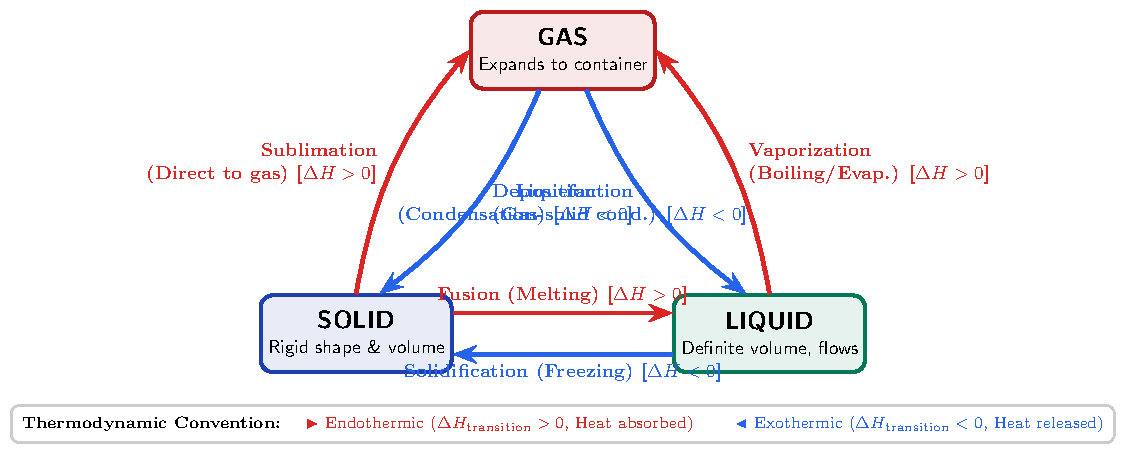
\includegraphics[width=0.88\textwidth]{figures/01_phase_transitions.pdf}
\caption{The thermodynamic cycle of macroscopic phase transitions. Red arrows denote endothermic transitions ($\Delta H > 0$, requiring thermal energy input); blue arrows denote exothermic transitions ($\Delta H < 0$, releasing thermal energy to the surroundings).}
\label{fig:phase_transitions}
\end{figure}

The six canonical phase transformations are classified in complementary forward-reverse pairs:
\begin{enumerate}[leftmargin=1.5em,itemsep=4pt]
  \item \textbf{Solid $\longleftrightarrow$ Liquid:}
  \begin{itemize}[leftmargin=1.2em]
    \item \textbf{Fusion (Melting):} Solid $\to$ Liquid. \emph{Endothermic} ($\Delta H_{\text{fus}} > 0$). Requires latent heat of fusion.
    \item \textbf{Solidification (Freezing):} Liquid $\to$ Solid. \emph{Exothermic} ($\Delta H_{\text{solid}} = -\Delta H_{\text{fus}} < 0$).
    \item At standard pressure ($P = 1\ \mathrm{atm}$), pure water melts/freezes at $T_{\text{fus}} = 0^\circ\mathrm{C}$ ($273.15\ \mathrm{K}$); pure iron melts at $T_{\text{fus}} = 1538^\circ\mathrm{C}$ ($1811\ \mathrm{K}$).
  \end{itemize}
  \item \textbf{Liquid $\longleftrightarrow$ Gas:}
  \begin{itemize}[leftmargin=1.2em]
    \item \textbf{Vaporization:} Liquid $\to$ Gas (by slow evaporation at the surface or boiling throughout the bulk). \emph{Endothermic} ($\Delta H_{\text{vap}} > 0$).
    \item \textbf{Liquefaction (Condensation):} Gas $\to$ Liquid. \emph{Exothermic} ($\Delta H_{\text{liq}} = -\Delta H_{\text{vap}} < 0$).
    \item Pure water boils at $T_{\text{vap}} = 100^\circ\mathrm{C}$ ($373.15\ \mathrm{K}$) at $1\ \mathrm{atm}$.
  \end{itemize}
  \item \textbf{Solid $\longleftrightarrow$ Gas:}
  \begin{itemize}[leftmargin=1.2em]
    \item \textbf{Sublimation:} Direct solid $\to$ gas transition without passing through an intermediate liquid phase. \emph{Endothermic} ($\Delta H_{\text{sub}} > 0$). Characteristic of dry ice ($\mathrm{CO_2}$ solid sublimates at $-78.5^\circ\mathrm{C}$) and iodine crystals ($\mathrm{I_2}$).
    \item \textbf{Deposition (Gas-Solid Condensation):} Direct gas $\to$ solid transition. \emph{Exothermic} ($\Delta H_{\text{dep}} = -\Delta H_{\text{sub}} < 0$). Observed in frost formation from water vapor.
  \end{itemize}
\end{enumerate}

By Hess's law of thermodynamic state functions, the enthalpy of sublimation equals the exact sum of fusion and vaporization enthalpies at identical temperature and pressure:
\begin{equation}
\Delta H_{\text{sub}} = \Delta H_{\text{fus}} + \Delta H_{\text{vap}}.
\end{equation}

\section{Physical vs. Chemical Changes and Lavoisier's Conservation Law}

\begin{definitionbox}{Physical Change vs. Chemical Change}
\begin{itemize}[leftmargin=1.5em,itemsep=3pt]
  \item \textbf{Physical Change:} A transformation that modifies the physical appearance, dimensions, or aggregation state of a substance, but leaves its \textbf{molecular and atomic constitution strictly invariant}. No chemical bonds are broken or created (e.g., dissolution of sugar in water, pulverization of rock salt, condensation of steam).
  \item \textbf{Chemical Change (Chemical Reaction):} A fundamental transformation wherein initial substances (\textbf{reactants}) are converted into chemically distinct new substances (\textbf{products}) via the rupture and reformation of electronic and chemical bonds.
\end{itemize}
\end{definitionbox}

Experimental indicators of a chemical transformation include:
\begin{enumerate}[leftmargin=1.5em,itemsep=2pt]
  \item Evolution of a gaseous product (effervescence),
  \item Formation of an insoluble solid precipitate ($\downarrow$),
  \item Permanent color change of the solution or solid matrix,
  \item Exothermic heat release ($\Delta H < 0$) or endothermic cooling ($\Delta H > 0$),
  \item Emission of electromagnetic radiation (chemiluminescence or flames).
\end{enumerate}

\begin{historicalbox}{Antoine-Laurent de Lavoisier: Father of Modern Chemistry}
\begin{minipage}{0.28\textwidth}
\centering
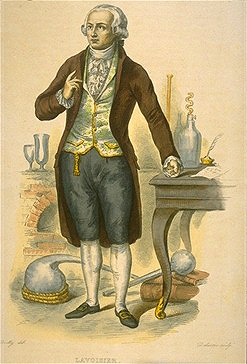
\includegraphics[width=0.92\textwidth]{images/lavoisier.jpg}
\captionof{figure}{Antoine-Laurent de Lavoisier (1743--1794), portrait by Jacques-Louis David (1788, Metropolitan Museum of Art).}
\end{minipage}\hfill
\begin{minipage}{0.68\textwidth}
In his revolutionary 1789 treatise \emph{Traité Élémentaire de Chimie}, French chemist Antoine-Laurent de Lavoisier dismantled the centuries-old phlogiston dogma. Utilizing closed hermetic combustion chambers and ultra-precise balance scales, Lavoisier demonstrated that during the combustion of phosphorus and sulfur in air, the weight gained by the solids was exactly equal to the weight lost by the surrounding air.

Lavoisier formulated the foundational axiom of chemistry: ``\emph{Rien ne se perd, rien ne se crée, tout se transforme}'' (Nothing is lost, nothing is created, everything is transformed), proving that chemical reactions represent a conserved atomic rearrangement.
\end{minipage}
\end{historicalbox}

\begin{lawbox}{Lavoisier's Law of Conservation of Mass}
In any closed chemical or physical system, the total mass remains strictly invariant throughout any transformation:
\begin{equation}
\sum m_{\text{reactants consumed}} = \sum m_{\text{products formed}}.
\end{equation}
In stoichiometric form for a general chemical reaction $\sum_i \nu_i \mathrm{R}_i \to \sum_j \nu_j' \mathrm{P}_j$:
\begin{equation}
\sum_i \nu_i M(\mathrm{R}_i) = \sum_j \nu_j' M(\mathrm{P}_j),
\end{equation}
which implies the strict, simultaneous conservation of every individual chemical element $X$.
\end{lawbox}

\section{Atoms, Molecules, and the Mole Concept}

\subsection{The Atomic and Molecular Nature of Matter}
\begin{itemize}[leftmargin=1.5em,itemsep=3pt]
  \item \textbf{The Atom:} The fundamental building block of chemical elements. An atom is electrically neutral, consisting of an ultra-dense, positively charged nucleus ($r_n \sim 10^{-14}\ \mathrm{m}$) surrounded by a diffuse cloud of negatively charged electrons ($r_{\text{atom}} \sim 10^{-10}\ \mathrm{m}$).
  \item \textbf{The Molecule:} A discrete, electrically neutral group of two or more atoms held together in a fixed spatial stoichiometry by covalent bonds (e.g., $\mathrm{H_2O, CO_2, NH_3}$).
\end{itemize}

\begin{historicalbox}{John Dalton and the Chemical Atomic Theory}
\begin{minipage}{0.28\textwidth}
\centering
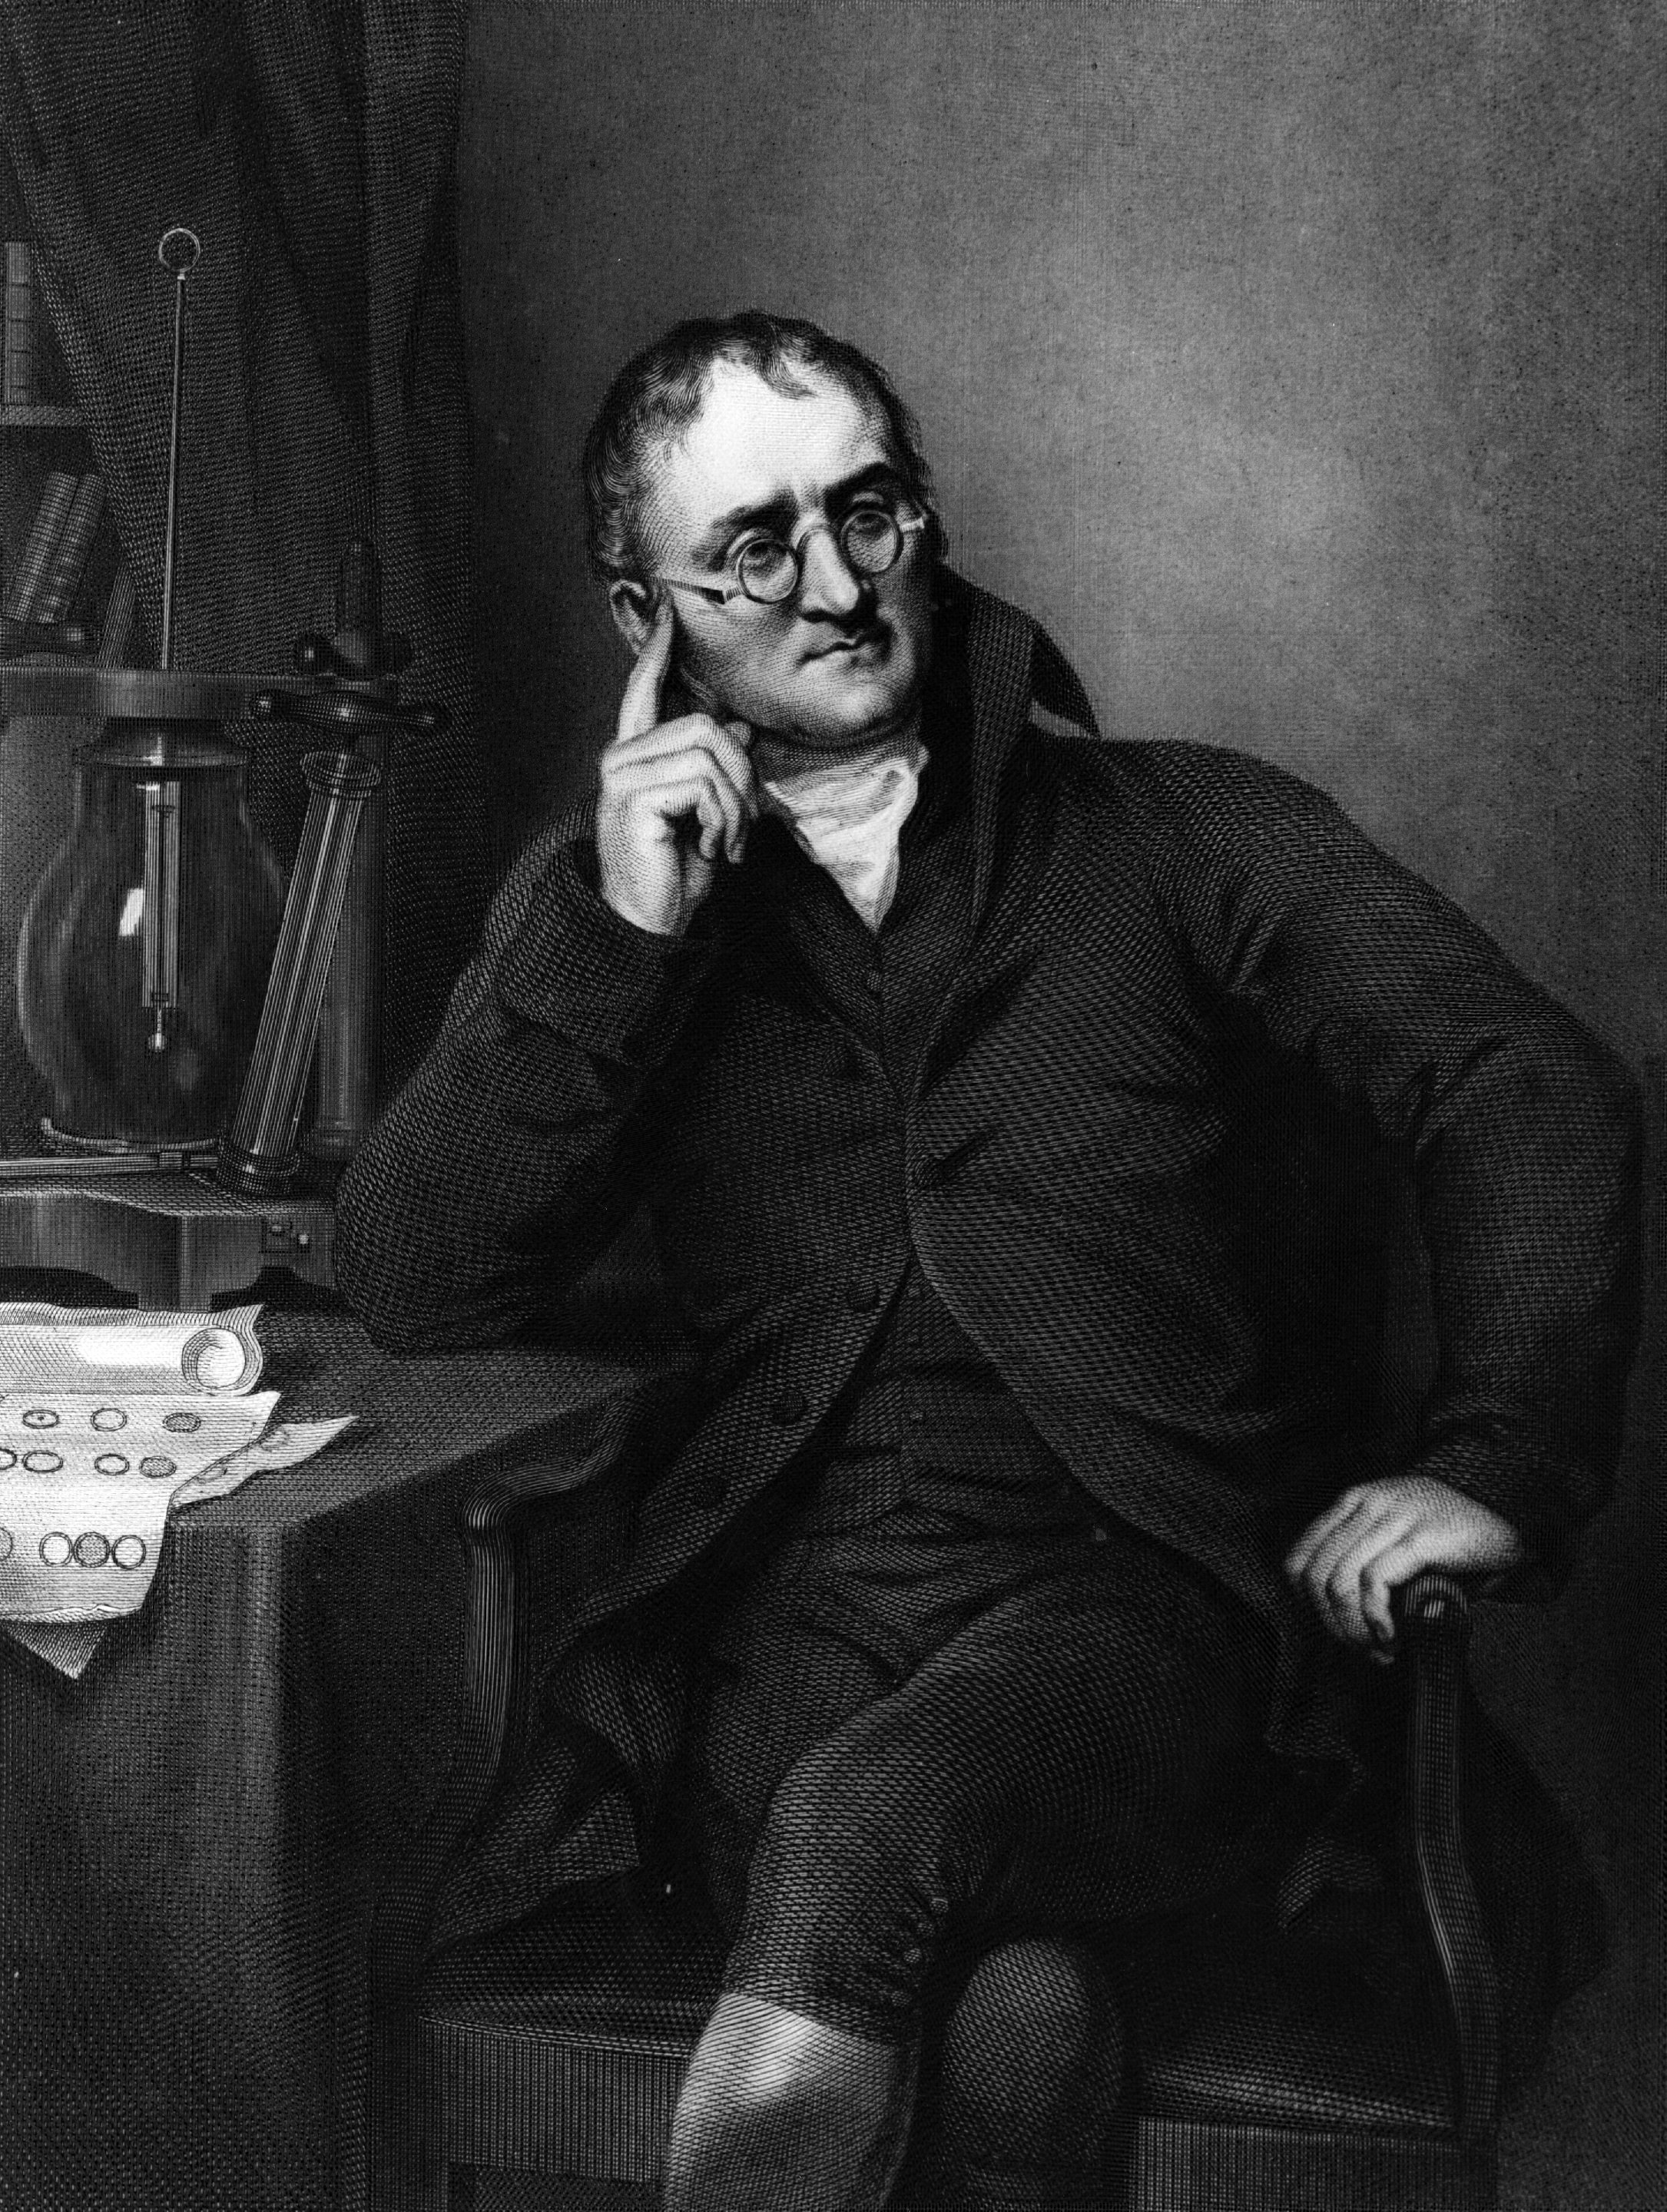
\includegraphics[width=0.92\textwidth]{images/dalton.jpg}
\captionof{figure}{John Dalton (1766--1844), portrait by Thomas Phillips (1835, National Portrait Gallery, London).}
\end{minipage}\hfill
\begin{minipage}{0.68\textwidth}
In 1803, English chemist and meteorologist John Dalton proposed the first modern atomic theory. Observing that elements always combine in fixed, simple integer mass ratios (the Law of Definite Proportions and the Law of Multiple Proportions), Dalton deduced that:
\begin{enumerate}[leftmargin=1.2em,itemsep=2pt]
  \item All matter consists of indivisible, indestructible particles called atoms;
  \item All atoms of a given element possess identical chemical properties and mass;
  \item Chemical compounds are formed when atoms of different elements combine in simple numerical ratios ($1:1, 1:2, 2:3$, etc.).
\end{enumerate}
\end{minipage}
\end{historicalbox}

\subsection{The Mole and Avogadro's Constant}

Because individual atoms have minuscule masses ($\sim 10^{-26}\ \mathrm{kg}$), macroscopic laboratory experiments require a bridge linking macroscopic mass measurements to microscopic particle counts.

\begin{definitionbox}{The Mole and Avogadro's Constant}
The \textbf{mole} (symbol: $\mathrm{mol}$) is the SI base unit for the \textbf{amount of substance} ($n$). One mole contains exactly $6.022\,140\,76 \times 10^{23}$ elementary entities (atoms, molecules, ions, electrons, or other specified groups of particles).
This defining numerical constant is \textbf{Avogadro's constant}:
\begin{equation}
N_A = 6.022\,140\,76 \times 10^{23}\ \mathrm{mol^{-1}} \quad (\text{often rounded to } 6.023 \times 10^{23}\ \mathrm{mol^{-1}}).
\end{equation}
The total number of particles $N$ in a sample of substance amount $n$ is:
\begin{equation}
N = n \cdot N_A \iff n = \frac{N}{N_A}.
\end{equation}
\end{definitionbox}

\begin{historicalbox}{Amedeo Avogadro and the Molecular Hypothesis}
\begin{minipage}{0.28\textwidth}
\centering
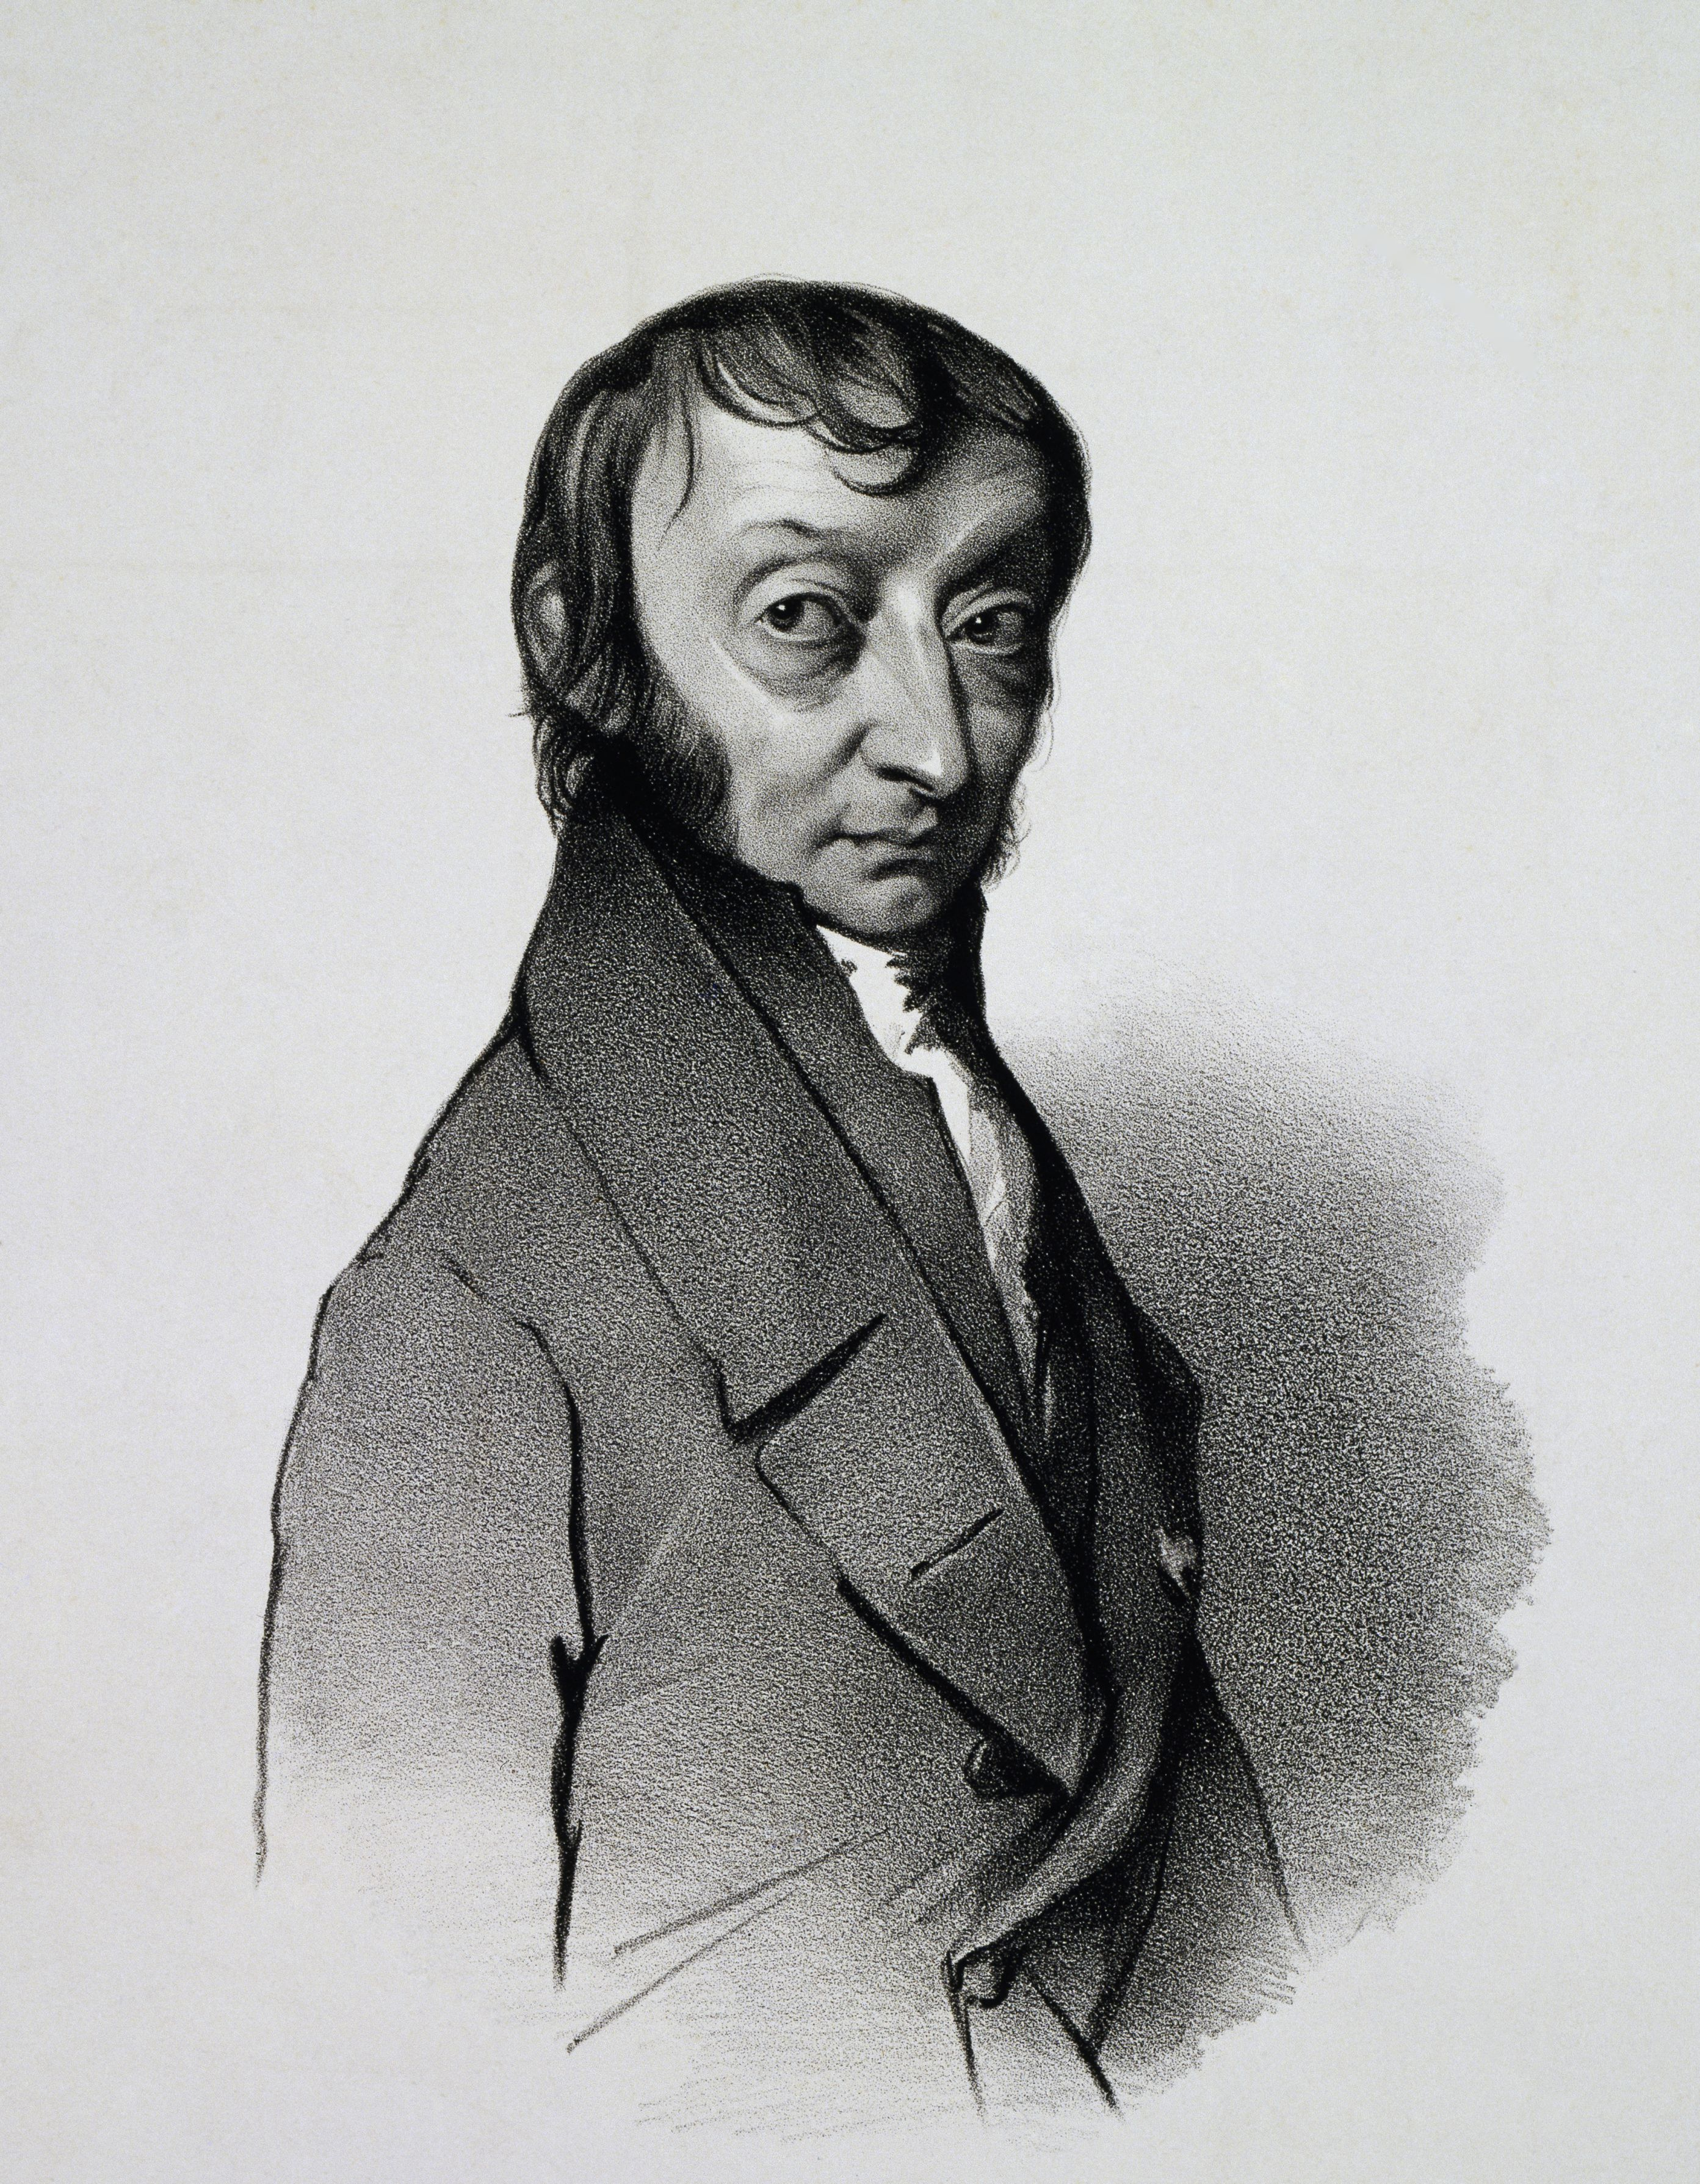
\includegraphics[width=0.92\textwidth]{images/avogadro.jpg}
\captionof{figure}{Amedeo Avogadro (1776--1856), contemporary Italian engraving.}
\end{minipage}\hfill
\begin{minipage}{0.68\textwidth}
In 1811, Italian physicist Amedeo Avogadro published his historic hypothesis: ``\emph{Equal volumes of all gases, measured at the same temperature and pressure, contain equal numbers of molecules}.''

Avogadro correctly distinguished between fundamental atoms and multi-atom molecules, explaining Gay-Lussac's law of combining volumes (e.g., $2\ \text{volumes of } \mathrm{H_2} + 1\ \text{volume of } \mathrm{O_2} \to 2\ \text{volumes of steam } \mathrm{H_2O}$). His brilliant insight was finally vindicated in 1860 by Stanislao Cannizzaro at the Karlsruhe Congress.
\end{minipage}
\end{historicalbox}

\section{Mass and Volume Metrics}

\subsection{1. The Unified Atomic Mass Unit}
Because the mass of an atom is inconveniently small in kilograms, the international scientific community defines an atomic-scale unit referenced to the carbon-12 isotope ($^{12}\mathrm{C}$):

\begin{definitionbox}{Unified Atomic Mass Unit (u or amu)}
The \textbf{unified atomic mass unit} ($1\ \mathrm{u}$) is defined as exactly $\frac{1}{12}$ of the mass of a single unbound, neutral Carbon-12 atom ($^{12}\mathrm{C}$) in its electronic and nuclear ground state:
\begin{equation}
1\ \mathrm{u} \eqdef \frac{1}{12} m(^{12}\mathrm{C}) = \frac{1}{N_A} \approx 1.660\,539 \times 10^{-24}\ \mathrm{g} = 1.660\,539 \times 10^{-27}\ \mathrm{kg}.
\end{equation}
\end{definitionbox}

\subsection{2. Molar Mass}
\begin{definitionbox}{Molar Mass ($M$)}
The \textbf{molar mass} $M$ of a substance is the mass of one mole ($N_A$ particles) of that substance:
\begin{equation}
M \eqdef \frac{m}{n}, \qquad [M] = \mathrm{g\cdot mol^{-1}} \quad (\text{or } \mathrm{kg\cdot mol^{-1}}).
\end{equation}
\begin{itemize}[leftmargin=1.5em,itemsep=2pt]
  \item \textbf{Atomic Molar Mass $M(X)$:} Mass of 1 mole of free atoms of element $X$. Numerically identical to its relative atomic mass in $\mathrm{u}$ (e.g., $M(\mathrm{H}) = 1.008\ \mathrm{g/mol}$, $M(\mathrm{C}) = 12.011\ \mathrm{g/mol}$, $M(\mathrm{O}) = 15.999\ \mathrm{g/mol}$, $M(\mathrm{S}) = 32.06\ \mathrm{g/mol}$).
  \item \textbf{Molecular Molar Mass $M(\mathrm{A}_x \mathrm{B}_y)$:} The stoichiometric sum of the atomic molar masses of all constituent atoms in the chemical formula:
  \begin{equation}
  M(\mathrm{A}_x \mathrm{B}_y) = x \cdot M(\mathrm{A}) + y \cdot M(\mathrm{B}).
  \end{equation}
  \emph{Example:} For water ($\mathrm{H_2O}$):
  \[
  M(\mathrm{H_2O}) = 2 M(\mathrm{H}) + M(\mathrm{O}) = 2(1.008) + 15.999 = 18.015\ \mathrm{g\cdot mol^{-1}}.
  \]
\end{itemize}
\end{definitionbox}

\subsection{3. Molar Volume of Gases}
\begin{definitionbox}{Molar Volume ($V_m$)}
The \textbf{molar volume} $V_m$ of a chemical substance is the spatial volume occupied by one mole of that substance in a specified thermodynamic state $(T, P)$:
\begin{equation}
V_m \eqdef \frac{V}{n}, \qquad [V_m] = \mathrm{L\cdot mol^{-1}} \quad (\text{or } \mathrm{m^3\cdot mol^{-1}}).
\end{equation}
From the Ideal Gas Law ($P V = n R T$):
\begin{equation}
V_m = \frac{R T}{P}.
\end{equation}
Under **Standard Temperature and Pressure (STP / CNTP)**, defined as $T_0 = 0^\circ\mathrm{C} = 273.15\ \mathrm{K}$ and $P_0 = 1\ \mathrm{atm} = 101\,325\ \mathrm{Pa}$:
\begin{equation}
V_m = \frac{(8.31446\ \mathrm{J\cdot mol^{-1}\cdot K^{-1}})(273.15\ \mathrm{K})}{101\,325\ \mathrm{Pa}} = 0.022\,414\ \mathrm{m^3\cdot mol^{-1}} = 22.414\ \mathrm{L\cdot mol^{-1}}.
\end{equation}
\end{definitionbox}

\begin{lawbox}{Universal Stoichiometric Master Equation}
For any pure chemical sample of mass $m$, particle count $N$, and gas volume $V_{\text{gas}}$ at STP:
\begin{equation}
n = \frac{m}{M} = \frac{N}{N_A} = \frac{V_{\text{gas}}}{V_m}.
\end{equation}
\end{lawbox}

\section{Classification of Matter and Solution Chemistry}

\subsection{Pure Substances and Mixtures}
Matter is universally partitioned into two great classes:

\begin{figure}[htbp]
\centering
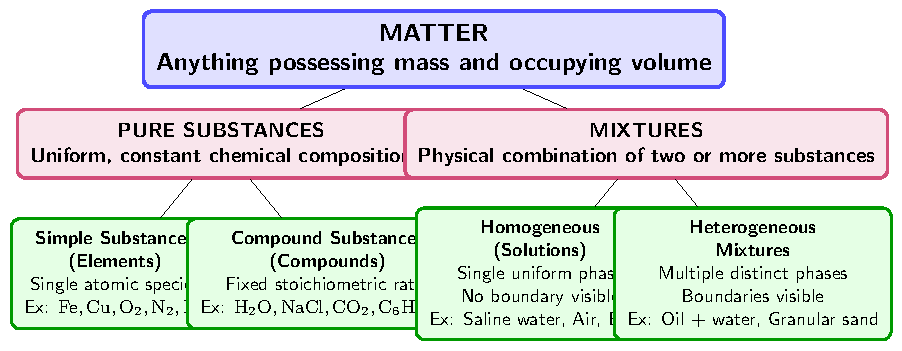
\includegraphics[width=0.88\textwidth]{figures/02_matter_classification.pdf}
\caption{The hierarchical classification of matter into pure substances (simple elements and compound species) and mixtures (homogeneous solutions and heterogeneous multi-phase systems).}
\label{fig:matter_classification}
\end{figure}

\begin{enumerate}[leftmargin=1.5em,itemsep=3pt]
  \item \textbf{Pure Substances:} Possess a uniform, definite, and invariant chemical composition throughout.
  \begin{itemize}[leftmargin=1.2em]
    \item \textbf{Simple Substances (Elements):} Formed from atoms of a single chemical element. Cannot be decomposed into simpler substances by chemical reactions (e.g., metals $\mathrm{Fe, Cu, Al}$; non-metal allotropes $\mathrm{O_2, O_3, C_{\text{graphite}}, S_8}$).
    \item \textbf{Compound Substances (Compounds):} Formed from two or more distinct elements chemically bound in fixed, constant stoichiometric proportions (e.g., $\mathrm{H_2O, NaCl, CO_2, H_2SO_4}$). Can be broken down into constituent elements by chemical reactions.
  \end{itemize}
  \item \textbf{Mixtures:} Physical combinations of two or more pure substances that do not react chemically. The components retain their individual chemical identities and can be separated by physical methods (distillation, filtration, centrifugation, chromatography).
  \begin{itemize}[leftmargin=1.2em]
    \item \textbf{Homogeneous Mixtures (Solutions):} The components are dispersed at the molecular or ionic scale, forming a single uniform macroscopic phase. No constituent boundaries are distinguishable, even under optical microscopy (e.g., sugar dissolved in water, air, bronze alloy).
    \item \textbf{Heterogeneous Mixtures:} Possess two or more distinct phases separated by visible interfaces. Constituents can be visually distinguished (e.g., oil and water, granite rock, suspension of clay in water).
  \end{itemize}
\end{enumerate}

\subsection{Solutions, Solutes, and Solvents}

\begin{definitionbox}{Solution Architecture}
A \textbf{solution} is a homogeneous mixture formed by dissolving one or more minor chemical species (\textbf{solutes}) into a predominant dispersing medium (\textbf{solvent}):
\begin{equation}
\text{Solution} = \text{Solvent} + \sum \text{Solutes}.
\end{equation}
When the solvent is liquid water ($\mathrm{H_2O}$), the system is designated an \textbf{aqueous solution}.
\end{definitionbox}

\begin{itemize}[leftmargin=1.5em,itemsep=3pt]
  \item \textbf{Solubility Limit and Saturation:} A solution is said to be \textbf{saturated} when the dissolved solute concentration has reached thermodynamic equilibrium with undissolved solute at a given temperature. Any additional solute cannot dissolve and settles as a solid precipitate ($\downarrow$), indicating \textbf{supersaturation}.
  \item \textbf{The Dilution Process:} Dilution consists of adding pure solvent to a pre-existing concentrated solution (\textbf{mother solution}), producing a lower-concentration \textbf{daughter solution}.
\end{itemize}

\begin{figure}[htbp]
\centering
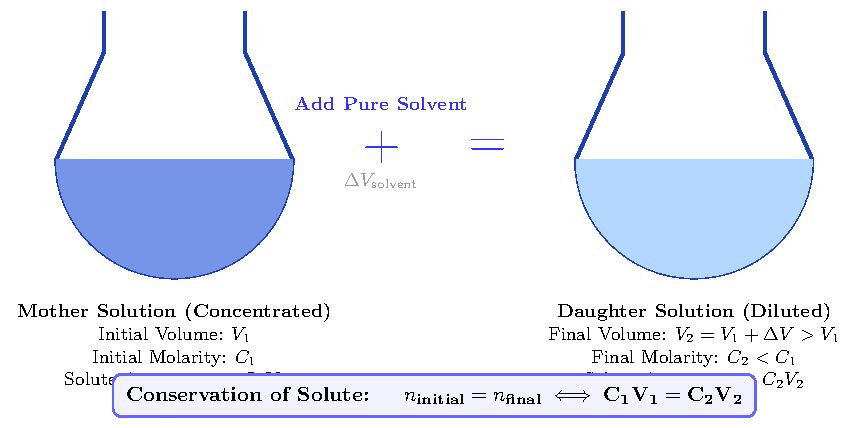
\includegraphics[width=0.88\textwidth]{figures/03_solution_dilution.pdf}
\caption{The principle of dilution. Adding pure solvent increases total volume from $V_1$ to $V_2$ while the absolute amount of dissolved solute remains strictly conserved ($n_1 = n_2 \implies C_1 V_1 = C_2 V_2$).}
\label{fig:solution_dilution}
\end{figure}

\begin{lawbox}{The Fundamental Dilution Invariant}
Because adding pure solvent adds strictly zero solute, the total amount of solute $n$ is an invariant of the dilution process:
\begin{equation}
n_{\text{initial}} = n_{\text{final}} \iff \mathbf{C_1 V_1 = C_2 V_2} \quad (\text{or } C_i V_i = C_f V_f).
\end{equation}
The dimensionless \textbf{dilution factor} $F$ is defined as:
\begin{equation}
F \eqdef \frac{V_2}{V_1} = \frac{C_1}{C_2} > 1.
\end{equation}
\end{lawbox}

\section{Mathematical Formulations of Solution Concentrations}

In chemistry, the composition of a solution is quantified through four standard concentration measures:

\subsection{1. Molarity (Molar Concentration, $C_M$ or $[\mathrm{X}]$)}
The molar concentration represents the amount of solute per unit volume of solution:
\begin{equation}
C_M \eqdef \frac{n_{\text{solute}}}{V_{\text{solution}}} = \frac{m_{\text{solute}}}{M_{\text{solute}} \cdot V_{\text{solution}}}, \qquad [C_M] = \mathrm{mol\cdot L^{-1}} = \mathrm{mol\cdot dm^{-3}} \equiv \mathrm{M}.
\end{equation}

\subsection{2. Mass Concentration (Titre or Mass Content, $C_m$)}
The mass concentration represents the mass of solute dissolved per unit volume of solution:
\begin{equation}
C_m \eqdef \frac{m_{\text{solute}}}{V_{\text{solution}}}, \qquad [C_m] = \mathrm{g\cdot L^{-1}}.
\end{equation}

\begin{lawbox}{Direct Relationship Between $C_m$ and $C_M$}
Multiplying molarity by the molar mass of the solute yields mass concentration directly:
\begin{equation}
C_m = \frac{m}{V} = \frac{n \cdot M}{V} = \left(\frac{n}{V}\right) M = \mathbf{C_M \cdot M}.
\end{equation}
\end{lawbox}

\subsection{3. Molality ($m$ or $b$)}
Molality expresses the amount of solute dissolved per unit mass of \textbf{pure solvent}:
\begin{equation}
m \eqdef \frac{n_{\text{solute}}}{m_{\text{solvent (in kg)}}}, \qquad [m] = \mathrm{mol\cdot kg^{-1}}.
\end{equation}
\emph{Crucial thermodynamic advantage:} Unlike molarity (which changes with temperature due to liquid thermal expansion $\dd V/\dd T \neq 0$), \textbf{molality is strictly independent of temperature and pressure}, making it the mandatory metric in colligative property thermodynamics (boiling-point elevation and freezing-point depression).

\subsection{4. Mass Fraction ($w$) and Percentage Purity ($P\%$)}
The mass fraction is the ratio of solute mass to total solution mass:
\begin{equation}
w \eqdef \frac{m_{\text{solute}}}{m_{\text{solution}}}, \qquad P\% \eqdef w \times 100\% = \frac{m_{\text{solute}}}{m_{\text{solution}}} \times 100\%.
\end{equation}
Given a concentrated commercial liquid solution of mass percentage $P\%$, solute molar mass $M$ ($\mathrm{g/mol}$), and relative density $d$ (specific gravity relative to water, $\rho = d\ \mathrm{g\cdot mL^{-1}} = 1000\,d\ \mathrm{g\cdot L^{-1}}$), the molarity is derived rigorously by considering $1\ \mathrm{L}$ ($1000\ \mathrm{mL}$) of solution:
\[
m_{\text{solution}} = 1000 \cdot d\ \mathrm{g}, \qquad m_{\text{solute}} = m_{\text{solution}} \times \frac{P\%}{100} = 10 \cdot d \cdot P\%\ \mathrm{g}.
\]
Dividing by molar mass $M$:
\begin{lawbox}{Molarity of Commercial Concentrated Reagents}
\begin{equation}
C_M = \frac{10 \cdot P\% \cdot d}{M}.
\end{equation}
\end{lawbox}

\subsection{5. Normality ($N$) and the Concept of Gram-Equivalents}

\begin{definitionbox}{Normality (Equivalent Concentration)}
The \textbf{normality} $N$ of a chemical solution is the number of **gram-equivalents** ($\mathrm{eq}$) of solute dissolved per liter of solution:
\begin{equation}
N \eqdef \frac{\text{Number of Gram-Equivalents}}{V_{\text{solution (L)}}}.
\end{equation}
The normality is related to molarity through the dimensionless stoichiometric **valence factor** $Z$:
\begin{equation}
\mathbf{N = C_M \cdot Z}.
\end{equation}
The unit of normality is the **equivalent per liter** ($\mathrm{eq\cdot L^{-1}}$ or $\mathrm{N}$).
\end{definitionbox}

The physical definition of the valence factor $Z$ depends strictly on the reaction context:

\begin{center}
\renewcommand{\arraystretch}{1.35}
\begin{tabular}{@{}lll@{}}
\toprule
\textbf{Reaction Context} & \textbf{Physical Definition of Valence Factor $Z$} & \textbf{Canonical Examples} \\
\midrule
\textbf{Acids} & Number of exchangeable acidic protons $\mathrm{H}^+$ & $\mathrm{HCl}: Z = 1 \implies N = C_M$ \\
& per formula unit & $\mathrm{H_2SO_4}: Z = 2 \implies N = 2 C_M$ \\
& & $\mathrm{H_3PO_4}: Z = 3 \implies N = 3 C_M$ \\
\midrule
\textbf{Bases} & Number of exchangeable hydroxide ions $\mathrm{OH}^-$ & $\mathrm{NaOH}: Z = 1 \implies N = C_M$ \\
& (or protons neutralized) per formula unit & $\mathrm{Ca(OH)_2}: Z = 2 \implies N = 2 C_M$ \\
& & $\mathrm{Al(OH)_3}: Z = 3 \implies N = 3 C_M$ \\
\midrule
\textbf{Salts} & Total positive charge: & $\mathrm{NaCl}: Z = 1 \times (+1) = 1$ \\
& (number of metal cations) $\times$ (cation charge) & $\mathrm{Na_2SO_4}: Z = 2 \times (+1) = 2$ \\
& & $\mathrm{Al_2(SO_4)_3}: Z = 2 \times (+3) = 6$ \\
\midrule
\textbf{Redox Reactions} & Number of electrons exchanged ($n_{e^-}$) & $\mathrm{MnO_4^-} \to \mathrm{Mn^{2+}} \ (5e^-): Z = 5$ \\
& in the specific half-reaction & $\mathrm{Cr_2O_7^{2-}} \to 2\mathrm{Cr^{3+}} \ (6e^-): Z = 6$ \\
& & $\mathrm{Fe^{2+}} \to \mathrm{Fe^{3+}} \ (1e^-): Z = 1$ \\
\bottomrule
\end{tabular}
\end{center}

\begin{lawbox}{The Equivalence Principle in Volumetric Titrations}
At the stoichiometric equivalence point of any quantitative volumetric titration between species 1 and species 2 (whether acid-base, precipitation, or redox), the number of reacting equivalents is identically equal:
\begin{equation}
N_1 V_1 = N_2 V_2.
\end{equation}
This universal equivalence law is the operational reason chemists introduced normality: it eliminates the need to carry stoichiometric coefficients explicitly during titration calculations.
\end{lawbox}

\begin{cautionbox}[Common Pitfall: Normality is Reaction-Dependent]
Unlike molarity, which is an intrinsic property of a prepared bottle, **normality depends on the reaction in which the substance participates**. For instance, in an acidic medium, potassium permanganate reacts via:
\[
\mathrm{MnO_4^-} + 8\mathrm{H}^+ + 5e^- \longrightarrow \mathrm{Mn}^{2+} + 4\mathrm{H_2O} \implies Z = 5 \implies N = 5 C_M.
\]
However, in a neutral or alkaline medium, it reduces only to manganese dioxide:
\[
\mathrm{MnO_4^-} + 2\mathrm{H_2O} + 3e^- \longrightarrow \mathrm{MnO_2} + 4\mathrm{OH}^- \implies Z = 3 \implies N = 3 C_M.
\]
A single $0.1\ \mathrm{M}\ \mathrm{KMnO_4}$ solution is $0.5\ \mathrm{N}$ in acid, but $0.3\ \mathrm{N}$ in base!
\end{cautionbox}

\section{Comprehensive Worked Examples}

\begin{workedexample}{Stoichiometric Combustion and Lavoisier Mass Conservation}
Propane gas ($\mathrm{C_3H_8}$) undergoes complete combustion with gaseous oxygen ($\mathrm{O_2}$) to produce carbon dioxide ($\mathrm{CO_2}$) and liquid water ($\mathrm{H_2O}$). A laboratory burner consumes $44.10\ \mathrm{g}$ of propane.
\begin{enumerate}[leftmargin=1.4em,itemsep=3pt]
  \item Write the balanced chemical equation and determine the stoichiometric mole ratios.
  \item Calculate the amount of substance (in moles) of propane consumed.
  \item Determine the theoretical mass of oxygen consumed, and the volume of pure oxygen and air required at STP ($V_m = 22.414\ \mathrm{L\cdot mol^{-1}}$, air is $21.0\%$ $\mathrm{O_2}$ by volume).
  \item Calculate the masses of $\mathrm{CO_2}$ and $\mathrm{H_2O}$ formed, and explicitly verify Lavoisier's conservation of mass.
\end{enumerate}

\paragraph{Solution.}
\textbf{1. Balanced Chemical Reaction:}\\
Balancing carbon ($3\ \mathrm{C}$), hydrogen ($8\ \mathrm{H} \to 4\ \mathrm{H_2O}$), and oxygen ($3 \times 2 + 4 \times 1 = 10\ \mathrm{O} \to 5\ \mathrm{O_2}$):
\[
\mathrm{C_3H_8(g)} + 5\,\mathrm{O_2(g)} \longrightarrow 3\,\mathrm{CO_2(g)} + 4\,\mathrm{H_2O(l)}.
\]

\textbf{2. Amount of Propane Consumed:}\\
The molar mass of propane is $M(\mathrm{C_3H_8}) = 3(12.011) + 8(1.008) = 36.033 + 8.064 = 44.097\ \mathrm{g\cdot mol^{-1}}$.
\[
n(\mathrm{C_3H_8}) = \frac{m}{M} = \frac{44.10\ \mathrm{g}}{44.097\ \mathrm{g\cdot mol^{-1}}} \approx 1.000\ \mathrm{mol}.
\]

\textbf{3. Oxygen Requirements:}\\
From the stoichiometric ratio $\frac{n(\mathrm{O_2})}{n(\mathrm{C_3H_8})} = \frac{5}{1}$:
\[
n(\mathrm{O_2}) = 5 \times 1.000 = 5.000\ \mathrm{mol}.
\]
The molar mass of oxygen is $M(\mathrm{O_2}) = 2(15.999) = 31.998\ \mathrm{g\cdot mol^{-1}}$.
The mass of oxygen consumed is:
\[
m(\mathrm{O_2}) = n \times M = 5.000\ \mathrm{mol} \times 31.998\ \mathrm{g\cdot mol^{-1}} = 159.99\ \mathrm{g} \approx 160.0\ \mathrm{g}.
\]
The volume of pure $\mathrm{O_2}$ gas required at STP is:
\[
V(\mathrm{O_2}) = n \times V_m = 5.000\ \mathrm{mol} \times 22.414\ \mathrm{L\cdot mol^{-1}} = 112.07\ \mathrm{L}.
\]
The corresponding volume of ambient air required is:
\[
V(\text{air}) = \frac{V(\mathrm{O_2})}{0.210} = \frac{112.07\ \mathrm{L}}{0.210} \approx 533.7\ \mathrm{L}.
\]

\textbf{4. Products Formed and Verification of Lavoisier Conservation:}\\
From the stoichiometry:
\begin{itemize}[leftmargin=1.5em,itemsep=3pt]
  \item Carbon dioxide: $n(\mathrm{CO_2}) = 3 \times 1.000 = 3.000\ \mathrm{mol}$.
  \[
  M(\mathrm{CO_2}) = 12.011 + 2(15.999) = 44.009\ \mathrm{g\cdot mol^{-1}}.
  \]
  \[
  m(\mathrm{CO_2}) = 3.000 \times 44.009 = 132.03\ \mathrm{g}.
  \]
  \item Water: $n(\mathrm{H_2O}) = 4 \times 1.000 = 4.000\ \mathrm{mol}$.
  \[
  M(\mathrm{H_2O}) = 2(1.008) + 15.999 = 18.015\ \mathrm{g\cdot mol^{-1}}.
  \]
  \[
  m(\mathrm{H_2O}) = 4.000 \times 18.015 = 72.06\ \mathrm{g}.
  \]
\end{itemize}
Total mass of reactants:
\[
\sum m_{\text{reactants}} = m(\mathrm{C_3H_8}) + m(\mathrm{O_2}) = 44.10\ \mathrm{g} + 159.99\ \mathrm{g} = 204.09\ \mathrm{g}.
\]
Total mass of products:
\[
\sum m_{\text{products}} = m(\mathrm{CO_2}) + m(\mathrm{H_2O}) = 132.03\ \mathrm{g} + 72.06\ \mathrm{g} = 204.09\ \mathrm{g}.
\]
The mass of products matches the mass of reactants to within $0.00\ \mathrm{g}$, rigorously illustrating Lavoisier's conservation law.
\end{workedexample}

\begin{workedexample}{Preparation of Diluted Reagent from Concentrated Commercial Acid}
A laboratory stock bottle of commercial nitric acid ($\mathrm{HNO_3}$) bears the following label specifications: mass percentage purity $P\% = 68.0\%$, relative density $d = 1.41$, and molar mass $M = 63.01\ \mathrm{g\cdot mol^{-1}}$.
\begin{enumerate}[leftmargin=1.4em,itemsep=3pt]
  \item Calculate the molarity ($C_{M1}$), mass concentration ($C_{m1}$), and normality ($N_1$) of the concentrated commercial nitric acid.
  \item Calculate the exact volume $V_1$ of commercial acid required to prepare $V_2 = 500.0\ \mathrm{mL}$ of a diluted solution of molarity $C_{M2} = 0.250\ \mathrm{mol\cdot L^{-1}}$.
  \item Describe the safe laboratory procedure for performing this dilution.
\end{enumerate}

\paragraph{Solution.}
\textbf{1. Commercial Acid Concentration Parameters:}\\
Applying the master formula for commercial liquid reagents:
\[
C_{M1} = \frac{10 \cdot P\% \cdot d}{M} = \frac{10 \times 68.0 \times 1.41}{63.01} = \frac{958.8}{63.01} \approx 15.216\ \mathrm{mol\cdot L^{-1}} \approx \mathbf{15.22\ \mathrm{M}}.
\]
The mass concentration is:
\[
C_{m1} = C_{M1} \cdot M = 15.216\ \mathrm{mol\cdot L^{-1}} \times 63.01\ \mathrm{g\cdot mol^{-1}} \approx 958.8\ \mathrm{g\cdot L^{-1}}.
\]
Because nitric acid is a strong monoprotic acid ($\mathrm{HNO_3} \to \mathrm{H}^+ + \mathrm{NO_3^-}$), each mole of $\mathrm{HNO_3}$ releases $Z = 1$ proton $\mathrm{H}^+$. Thus:
\[
N_1 = C_{M1} \cdot Z = 15.22 \times 1 = \mathbf{15.22\ \mathrm{N}}.
\]

\textbf{2. Required Aliquot Volume $V_1$:}\\
Applying the dilution conservation law $C_{M1} V_1 = C_{M2} V_2$:
\[
V_1 = \frac{C_{M2} V_2}{C_{M1}} = \frac{0.250\ \mathrm{mol\cdot L^{-1}} \times 500.0\ \mathrm{mL}}{15.216\ \mathrm{mol\cdot L^{-1}}} = \frac{125.0}{15.216} \approx \mathbf{8.215\ \mathrm{mL}}.
\]
The chemist must withdraw exactly $8.22\ \mathrm{mL}$ of the concentrated commercial acid.

\textbf{3. Safety Laboratory Protocol:}\\
Dilution of concentrated strong mineral acids is highly exothermic. \textbf{Never pour water into concentrated acid} (risk of violent boiling, splattering, and acid burns).
The safe protocol is:
\begin{itemize}[leftmargin=1.5em,itemsep=2pt]
  \item Fill a $500\ \mathrm{mL}$ volumetric flask roughly halfway ($\sim 250\ \mathrm{mL}$) with deionized water;
  \item Using a calibrated volumetric pipette and propipette bulb inside a fume hood, slowly dispense $8.22\ \mathrm{mL}$ of commercial nitric acid down the neck into the water;
  \item Swirl gently to dissipate heat;
  \item Allow the flask to cool to room temperature ($20^\circ\mathrm{C}$);
  \item Add deionized water dropwise using a wash bottle until the bottom of the meniscus aligns precisely with the calibration mark;
  \item Stopper the flask and invert several times to ensure total homogeneity.
\end{itemize}
\end{workedexample}

\begin{workedexample}{Redox Normality and Volumetric Titration Equivalence}
A volumetric analysis is performed to determine the concentration of iron(II) sulfate ($\mathrm{FeSO_4}$) in an acidic aqueous solution. An aliquot of $V_{\text{Fe}} = 20.00\ \mathrm{mL}$ of the $\mathrm{FeSO_4}$ solution requires $V_{\text{ox}} = 16.40\ \mathrm{mL}$ of a $0.0200\ \mathrm{M}$ potassium permanganate ($\mathrm{KMnO_4}$) standard solution to reach the faint permanent pink equivalence point.
\begin{enumerate}[leftmargin=1.4em,itemsep=3pt]
  \item Write the balanced redox half-reactions and the overall ionic equation in acidic medium.
  \item Determine the valence factor $Z$ and the normality $N_{\text{ox}}$ of the $\mathrm{KMnO_4}$ solution.
  \item Using the equivalence principle $N_1 V_1 = N_2 V_2$, determine the normality $N_{\text{Fe}}$ and molarity $C_{M,\text{Fe}}$ of the $\mathrm{FeSO_4}$ solution.
  \item Compute the mass concentration $C_{m,\mathrm{FeSO_4}}$ of iron(II) sulfate ($M = 151.91\ \mathrm{g\cdot mol^{-1}}$).
\end{enumerate}

\paragraph{Solution.}
\textbf{1. Redox Half-Reactions and Balanced Equation:}\\
The two redox half-reactions in acidic solution are:
\begin{align*}
\text{Reduction (Oxidant):} \quad & \mathrm{MnO_4^-} + 8\,\mathrm{H}^+ + 5\,e^- \longrightarrow \mathrm{Mn}^{2+} + 4\,\mathrm{H_2O} \\
\text{Oxidation (Reductant):} \quad & \mathrm{Fe}^{2+} \longrightarrow \mathrm{Fe}^{3+} + 1\,e^-
\end{align*}
Multiplying the iron oxidation half-reaction by $5$ to balance electrons:
\[
\mathrm{MnO_4^-} + 5\,\mathrm{Fe}^{2+} + 8\,\mathrm{H}^+ \longrightarrow \mathrm{Mn}^{2+} + 5\,\mathrm{Fe}^{3+} + 4\,\mathrm{H_2O}.
\]

\textbf{2. Valence Factors and Normality of $\mathrm{KMnO_4}$:}\\
In this acidic reaction, the permanganate ion captures $5$ electrons. Therefore:
\[
Z_{\text{ox}} = 5 \implies N_{\text{ox}} = C_{M,\text{ox}} \cdot Z_{\text{ox}} = 0.0200\ \mathrm{mol\cdot L^{-1}} \times 5 = \mathbf{0.1000\ \mathrm{N}}.
\]

\textbf{3. Determination of Iron Concentration:}\\
At the titration equivalence point, the number of gram-equivalents of oxidant and reductant are identically equal:
\[
N_{\text{Fe}} V_{\text{Fe}} = N_{\text{ox}} V_{\text{ox}} \implies N_{\text{Fe}} = \frac{N_{\text{ox}} V_{\text{ox}}}{V_{\text{Fe}}}.
\]
Plugging in the titration volumes:
\[
N_{\text{Fe}} = \frac{0.1000\ \mathrm{eq\cdot L^{-1}} \times 16.40\ \mathrm{mL}}{20.00\ \mathrm{mL}} = \mathbf{0.0820\ \mathrm{eq\cdot L^{-1}} = 0.0820\ \mathrm{N}}.
\]
In the oxidation half-reaction, each $\mathrm{Fe}^{2+}$ ion transfers $Z_{\text{Fe}} = 1$ electron ($\mathrm{Fe}^{2+} \to \mathrm{Fe}^{3+} + 1e^-$). Therefore:
\[
C_{M,\text{Fe}} = \frac{N_{\text{Fe}}}{Z_{\text{Fe}}} = \frac{0.0820\ \mathrm{N}}{1} = \mathbf{0.0820\ \mathrm{mol\cdot L^{-1}} = 0.0820\ \mathrm{M}}.
\]
Notice how effortlessly normality resolved the $1:5$ stoichiometric ratio without needing to juggle mole fractions!

\textbf{4. Mass Concentration:}\\
The mass concentration of dissolved anhydrous $\mathrm{FeSO_4}$ is:
\[
C_{m} = C_M \cdot M = 0.0820\ \mathrm{mol\cdot L^{-1}} \times 151.91\ \mathrm{g\cdot mol^{-1}} = \mathbf{12.46\ \mathrm{g\cdot L^{-1}}}.
\]
\end{workedexample}

\begin{workedexample}{Multi-Step Dilution and Mixing of Solutions}
A chemist mixes $V_1 = 200.0\ \mathrm{mL}$ of an aqueous sulfuric acid solution of molarity $C_{M1} = 0.500\ \mathrm{M}$ with $V_2 = 300.0\ \mathrm{mL}$ of a sulfuric acid solution of molarity $C_{M2} = 0.200\ \mathrm{M}$. The combined mixture is subsequently transferred to a volumetric flask and diluted with deionized water to a final volume of $V_{\text{final}} = 1.000\ \mathrm{L}$.
\begin{enumerate}[leftmargin=1.4em,itemsep=3pt]
  \item Determine the total amount of sulfuric acid ($\mathrm{H_2SO_4}$) present in the final mixture.
  \item Compute the final molarity ($C_{M,\text{final}}$), mass concentration ($C_{m,\text{final}}$), and normality ($N_{\text{final}}$) of the prepared solution ($M(\mathrm{H_2SO_4}) = 98.08\ \mathrm{g\cdot mol^{-1}}$).
\end{enumerate}

\paragraph{Solution.}
\textbf{1. Total Amount of Substance:}\\
The total amount of $\mathrm{H_2SO_4}$ solute is the sum of moles contributed by solution 1 and solution 2:
\[
n_1 = C_{M1} \cdot V_1 = 0.500\ \mathrm{mol\cdot L^{-1}} \times 0.2000\ \mathrm{L} = 0.1000\ \mathrm{mol},
\]
\[
n_2 = C_{M2} \cdot V_2 = 0.200\ \mathrm{mol\cdot L^{-1}} \times 0.3000\ \mathrm{L} = 0.0600\ \mathrm{mol}.
\]
The total amount of solute is:
\[
n_{\text{total}} = n_1 + n_2 = 0.1000 + 0.0600 = \mathbf{0.1600\ \mathrm{mol}}.
\]

\textbf{2. Final Concentrations:}\\
The final volume of the solution is $V_{\text{final}} = 1.000\ \mathrm{L}$.
\begin{itemize}[leftmargin=1.5em,itemsep=3pt]
  \item \textbf{Final Molarity:}
  \[
  C_{M,\text{final}} = \frac{n_{\text{total}}}{V_{\text{final}}} = \frac{0.1600\ \mathrm{mol}}{1.000\ \mathrm{L}} = \mathbf{0.1600\ \mathrm{mol\cdot L^{-1}} = 0.1600\ \mathrm{M}}.
  \]
  \item \textbf{Final Mass Concentration:}
  \[
  C_{m,\text{final}} = C_{M,\text{final}} \cdot M = 0.1600\ \mathrm{mol\cdot L^{-1}} \times 98.08\ \mathrm{g\cdot mol^{-1}} = \mathbf{15.69\ \mathrm{g\cdot L^{-1}}}.
  \]
  \item \textbf{Final Normality:}
  Sulfuric acid is a diprotic acid ($\mathrm{H_2SO_4} \to 2\mathrm{H}^+ + \mathrm{SO_4^{2-}}$), releasing $Z = 2$ protons $\mathrm{H}^+$ per molecule upon complete neutralization. Therefore:
  \[
  N_{\text{final}} = C_{M,\text{final}} \cdot Z = 0.1600\ \mathrm{M} \times 2 = \mathbf{0.3200\ \mathrm{N}}.
  \]
\end{itemize}
\end{workedexample}
